% Options for packages loaded elsewhere
\PassOptionsToPackage{unicode}{hyperref}
\PassOptionsToPackage{hyphens}{url}
%
\documentclass[t,aspectratio=169]{beamer}
% \documentclass[
    % ignorenonframetext,
% ]{beamer}
    
\usepackage{beamerthemetue2018}
\usepackage{listings}
\usepackage{mdframed} % surround environments with tags
\usepackage[outputdir=build]{minted} % code snippet colors
\usemintedstyle{xcode}
 
\usepackage{csquotes}
\usepackage[english]{babel}

\usepackage{graphicx}                   % For images
% \usepackage{pandocMarkdown} % internal package wrapping glosseries
 

% \usepackage[
%     contentBlocks,
%     debugExtensions,
%     definitionLists,
%     fancy_lists,
%     fencedCode,
%     hashEnumerators,
%     inlineNotes,
%     jekyllData,
%     expectJekyllData=false,
%     notes,
%     pipeTables,
%     rawAttribute,
%     headerAttributes,
%     smartEllipses,
%     strikeThrough,
%     subscripts,
%     superscripts,
%     tableCaptions,
%     taskLists,
%     citations,
%     hybrid,
%     relativeReferences,
%     texComments,
%     stripIndent,
%     underscores=false,
%     outputDir=build,
%     % theme=witiko/graphicx/http,
%     % theme=witiko/beamer/MU,
% ]{markdown} 
% \def\markdownOptionOutputDir{build}
 
\graphicspath{
  {./figures/}
}

 
\mode<presentation>

\title{Secure Sessions for Ad Hoc Multiparty Computation in MPyC}
\subtitle{Master thesis preparation phase}
% \author{Emil Nikolov \\ Id nr: 0972305 \\ emil.e.nikolov@gmail.com}
\author{Emil Nikolov \\ Id nr: 0972305 \\ emil.e.nikolov@gmail.com \\ Supervisor: Dr. ir. L.A.M. (Berry) Schoenmakers}
% \author{Emil Nikolov Id nr: 0972305  emil.e.nikolov@gmail.com  Supervisor: Dr. ir. L.A.M. (Berry) Schoenmakers}
% \supervisor{Dr. ir. L.A.M. (Berry) Schoenmakers}
\department{Department of Mathematics and Computer Science}
% \documentclass{article}
% \def\exec{\immediate\write18}
% \def\inputAllFiles#1{%
%   \def\filename{build/\jobname.md}
%   \exec{for i in #1/*.md; do echo >> \filename && cat $i >> \filename && echo >> \filename && echo >> \filename;done}%
%   % \exec{for i in #1/*.md; do cat $i >> \filename; done}%
%   \markdownInput{\filename}
%   \AtEndDocument{\exec{cp -f build/\jobname.md #1/\jobname.tmp; rm -f build/\jobname.md}}
% }

\usepackage{pandocBeamer} % internal package wrapping glosseries
\begin{document}


\let\inputmintedorg\inputminted
\renewcommand{\inputminted}[2]{%
  \begin{mdframed}
    \inputmintedorg[linenos=true,fontsize=\tiny,breaklines=true,breakanywhere=true]{#1}{#2}
  \end{mdframed}
}

\begin{titleframe}[variant=1,bgimage=titlebgimg.jpg]
\end{titleframe}

\title{}


\begin{frame}
  \frametitle{Outline}
  \tableofcontents
\end{frame}

\setkeys{Gin}{scale=0.25}

\begin{frame}
\section{Introduction}
\end{frame}

\begin{frame}{Introduction}
\protect\hypertarget{introduction}{}
What is Secure Multiparty Computation?

\begin{itemize}
\tightlist
\item
  Joint computation of a function
\item
  Secret inputs
\item
  Only final result is revealed
\end{itemize}

Examples:

\begin{itemize}
\tightlist
\item
  Millionaire's problem
\item
  Secret Santa
\item
  Electronic voting
\item
  Auctions
\item
  Machine learning
\end{itemize}
\end{frame}

\begin{frame}{MPC Basics}
\protect\hypertarget{mpc-basics}{}
\begin{itemize}
\tightlist
\item
  Lagrange Interpolation

  \begin{itemize}
  \tightlist
  \item
    Set of \(t+1\) points uniquely identify a polynomial of degree
    \(\leq t\)
  \end{itemize}
\item
  Shamir's Secret Sharing

  \begin{itemize}
  \tightlist
  \item
    \((t, m)\)-threshold secret sharing scheme based on Lagrange
    Interpolation
  \item
    \(\geq\) \(t+1\) shares to reconstruct the secret \(S\)
  \item
    Choose random polynomial \(f(x)\) of degree \(t\) where \(f(0) = S\)
  \item
    Share \(s_i = f(i)\), for \(i \in [1,m]\)
  \end{itemize}
\item
  Secure Multiparty Computation

  \begin{itemize}
  \tightlist
  \item
    \(m\) parties jointly compute a function
    \(f(S_{1},S_{2},\dots,S_{m})\), from their secret inputs
  \item
    Party \(i\) secret shares its private input \(S_{i}\) with the
    others
  \item
    Interactive protocol to reconstruct a polynomial \(g(x)\), where
    \(g(0)=f(S_1, S_2, \dots, S_m)\)
  \end{itemize}
\end{itemize}
\end{frame}

\begin{frame}{Problem Description}
\protect\hypertarget{problem-description}{}
MPyC:

\begin{itemize}
\tightlist
\item
  Python framework for MPC developed at TU/e
\item
  No service discovery yet
\item
  Target users of different level of expertise

  \begin{itemize}
  \tightlist
  \item
    Casual
  \item
    Power
  \item
    Enterprise
  \end{itemize}
\item
  MPC is Peer-to-Peer
\item
  Local networks are tricky

  \begin{itemize}
  \tightlist
  \item
    Limited supply of IPv4 addresses
  \item
    Slow adoption of IPv6
  \item
    Network Address Translation (NAT)
  \end{itemize}
\end{itemize}
\end{frame}

\begin{frame}{Research Questions}
\protect\hypertarget{research-questions}{}
\emph{How can MPyC be extended to enable casual users, power users and
enterprises with limited prior knowledge of each other to discover each
other and perform a secure multiparty computation under diverse
networking conditions?}

\begin{itemize}
\tightlist
\item
  deployment strategies?
\item
  identity?
\item
  first contact?
\item
  connectivity?

  \begin{itemize}
  \tightlist
  \item
    security?
  \item
    privacy?
  \item
    performance?
  \end{itemize}
\end{itemize}
\end{frame}

\begin{frame}{Preparation Phase Scope}
\protect\hypertarget{preparation-phase-scope}{}
\begin{itemize}
\tightlist
\item
  Technical Survey
\item
  Extensible Evaluation Environment (\(E^3\)) - network of host machines
  for MPC

  \begin{itemize}
  \tightlist
  \item
    Simple
  \item
    Extensible
  \item
    Cross region
  \item
    Cross platform
  \item
    Automated
  \item
    Reproducible
  \item
    Disposable
  \end{itemize}
\item
  Implementation Phase Planning
\end{itemize}
\end{frame}

\begin{frame}{}
\protect\hypertarget{section}{}
\section{Technical Survey}
\end{frame}

\begin{frame}{Technical Survey}
\protect\hypertarget{technical-survey}{}
\begin{itemize}
\tightlist
\item
  Deployment tools
\item
  Connectivity approaches
\end{itemize}
\end{frame}

\begin{frame}{Infrastructure as Code (IaC)}
\protect\hypertarget{infrastructure-as-code-iac}{}
Tools:

\begin{itemize}
\tightlist
\item
  Provisioning - Terraform, CloudFormation
\item
  Deployment - Ansible, Puppet, Chef
\end{itemize}

Specification:

\begin{itemize}
\tightlist
\item
  Imperative - describes the steps to execute
\item
  Declarative - describes the desired state
\end{itemize}

Operating Systems:

\begin{itemize}
\tightlist
\item
  Most Linux distributions are imperatively managed
\item
  NixOS

  \begin{itemize}
  \tightlist
  \item
    Declarative
  \item
    Deployment tools: NixOps, Colmena, morph, deploy-rs
  \end{itemize}
\end{itemize}
\end{frame}

\begin{frame}{Virtual Private Networks (VPNs)}
\protect\hypertarget{virtual-private-networks-vpns}{}
\begin{itemize}
\tightlist
\item
  Centralized VPNs - OpenVPN, IPSec

  \begin{itemize}
  \tightlist
  \item
    Emulate a real network
  \item
    Transparent to the other programs on the host
  \item
    Single point of failure
  \item
    Can be bottlenecked
  \end{itemize}
\item
  Mesh VPNs - Tailscale, Nebula, Tinc

  \begin{itemize}
  \tightlist
  \item
    Peer-to-Peer traffic
  \item
    Discovery can happen via a public service or from a known peer
  \end{itemize}
\end{itemize}
\end{frame}

\begin{frame}{Network Address Translation (NAT)}
\protect\hypertarget{network-address-translation-nat}{}
\begin{columns}[T]
\begin{column}{0.48\textwidth}
\begin{figure}
\centering
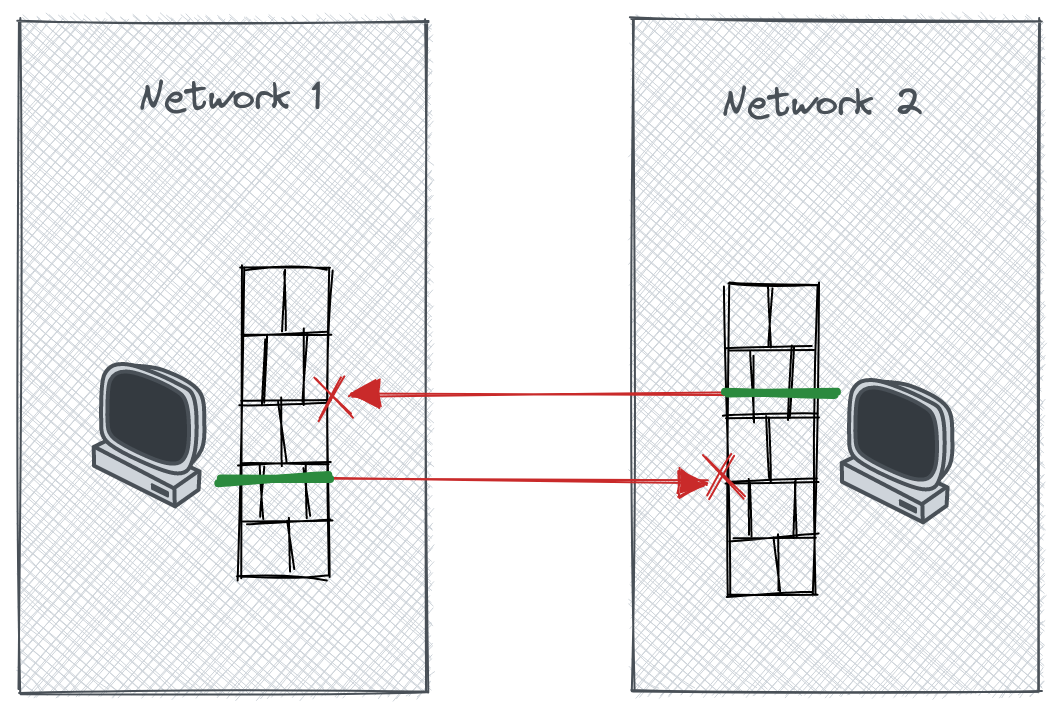
\includegraphics[width=\textwidth,height=0.66\textheight]{presentation/../figures/nat-intro.png}
\caption{``Two parties behind separate NATs''\label{nat-intro}}
\end{figure}
\end{column}

\begin{column}{0.48\textwidth}
\begin{itemize}
\tightlist
\item
  Parties behind a NAT device (usually their router)

  \begin{itemize}
  \tightlist
  \item
    Can initiate a connection to a public endpoint
  \item
    Cannot be discovered from the outside
  \item
    Neither party can initiate the connection to the other
  \end{itemize}
\end{itemize}
\end{column}
\end{columns}
\end{frame}

\begin{frame}{NAT Traversal}
\protect\hypertarget{nat-traversal}{}
\begin{columns}[T]
\begin{column}{0.48\textwidth}
\begin{figure}
\centering
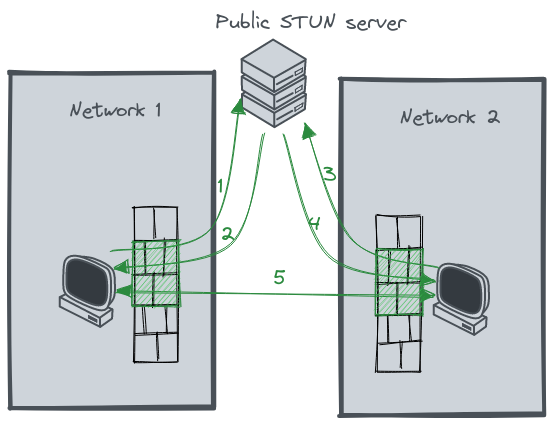
\includegraphics[width=\textwidth,height=0.66\textheight]{presentation/../figures/nat-traversal.png}
\caption{``NAT traversal via STUN''\label{nat-traversal}}
\end{figure}
\end{column}

\begin{column}{0.48\textwidth}
\begin{itemize}
\tightlist
\item
  Session Traversal Utilities for NAT (STUN)

  \begin{itemize}
  \tightlist
  \item
    Parties connect to a public STUN server (can be another party)
  \item
    The server reports the IPs it ``sees'' the parties at
  \item
    User Datagram Protocol (UDP) hole punching

    \begin{itemize}
    \tightlist
    \item
      Reverse channel for the STUN server to talk back to a party
    \item
      Appropriated by the other parties for their own traffic
    \end{itemize}
  \end{itemize}
\end{itemize}
\end{column}
\end{columns}
\end{frame}

\begin{frame}{Other approaches}
\protect\hypertarget{other-approaches}{}
\begin{itemize}
\tightlist
\item
  Decentralized identifiers (DIDs) and DIDComm

  \begin{itemize}
  \tightlist
  \item
    Lack of sessions
  \item
    Inefficient for MPC
  \end{itemize}
\item
  The Onion Router

  \begin{itemize}
  \tightlist
  \item
    Privacy
  \item
    Onion services
  \end{itemize}
\item
  Peer-to-peer applications

  \begin{itemize}
  \tightlist
  \item
    Bit Torrents
  \item
    Ethereum
  \item
    IPFS
  \end{itemize}
\end{itemize}
\end{frame}

\begin{frame}{}
\protect\hypertarget{section}{}
\section{Reference Implementation}
\end{frame}

\begin{frame}{Reference Implementation}
\protect\hypertarget{reference-implementation}{}
\begin{itemize}
\tightlist
\item
  DigitalOcean - cloud provider
\item
  RaspberryPi - ARM based Single Board Computer (SBC)
\item
  NixOS - declarative Linux distribution
\item
  Terraform - declarative provisioning
\item
  Colmena - declarative NixOS deployment
\item
  Tailscale - mesh VPN as a Service
\item
  prsync - sync directories to multiple hosts over ssh
\item
  pssh - execute commands on multiple hosts in parallel over ssh
\end{itemize}
\end{frame}

\begin{frame}[fragile]{Nix - Basic flake.nix}
\protect\hypertarget{nix---basic-flake.nix}{}
\begin{Shaded}
\begin{Highlighting}[]
\OperatorTok{\{}
  \VariableTok{inputs} \OperatorTok{=} \OperatorTok{\{}
    \VariableTok{nixpkgs}\NormalTok{.}\VariableTok{url} \OperatorTok{=} \StringTok{"github:nixos/nixpkgs/nixos{-}unstable"}\OperatorTok{;}
  \OperatorTok{\};}

  \VariableTok{outputs} \OperatorTok{=}\NormalTok{ inputs@}\OperatorTok{\{} \VariableTok{self}\OperatorTok{,} \VariableTok{nixpkgs}\OperatorTok{,} \OperatorTok{...} \OperatorTok{\}}\NormalTok{:}
    \KeywordTok{let}
      \VariableTok{pkgs} \OperatorTok{=} \BuiltInTok{import}\NormalTok{ nixpkgs }\OperatorTok{\{}
        \VariableTok{system} \OperatorTok{=} \StringTok{"x86\_64{-}linux"}\OperatorTok{;}
      \OperatorTok{\};}
    \KeywordTok{in}
    \OperatorTok{\{}
        \VariableTok{myHello} \OperatorTok{=}\NormalTok{ pkgs.hello}\OperatorTok{;}
    \OperatorTok{\};}
\OperatorTok{\}}
\end{Highlighting}
\end{Shaded}
\end{frame}

\begin{frame}[fragile]{Nix - flake.lock}
\protect\hypertarget{nix---flake.lock}{}
\begin{Shaded}
\begin{Highlighting}[]
\OperatorTok{\{}
  \StringTok{"}\NormalTok{nodes}\StringTok{"}\NormalTok{: \{}
    \StringTok{"nixpkgs"}\NormalTok{: \{}
      \StringTok{"locked"}\NormalTok{: \{}
        \StringTok{"lastModified"}\NormalTok{: 1666377499,}
        \StringTok{"narHash"}\NormalTok{: }\StringTok{"sha256{-}dZZCGvWcxc7oGnUgFVf0UeNHsJ4VhkTM0v5JRe8EwR8="}\NormalTok{,}
        \StringTok{"owner"}\NormalTok{: }\StringTok{"nixos"}\NormalTok{,}
        \StringTok{"repo"}\NormalTok{: }\StringTok{"nixpkgs"}\NormalTok{,}
        \StringTok{"rev"}\NormalTok{: }\StringTok{"301aada7a64812853f2e2634a530ef5d34505048"}\NormalTok{,}
        \StringTok{"type"}\NormalTok{: }\StringTok{"github"}
      \OperatorTok{\}}\NormalTok{,}
      \StringTok{"original"}\NormalTok{: }\OperatorTok{\{}
        \StringTok{"}\NormalTok{owner}\StringTok{"}\NormalTok{: }\StringTok{"nixos"}\NormalTok{,}
        \StringTok{"ref"}\NormalTok{: }\StringTok{"nixos{-}unstable"}\NormalTok{,}
        \StringTok{"repo"}\NormalTok{: }\StringTok{"nixpkgs"}\NormalTok{,}
        \StringTok{"type"}\NormalTok{: }\StringTok{"github"}
      \OperatorTok{\}}
\NormalTok{    \},}
\NormalTok{    ...}
\NormalTok{  \}}
\NormalTok{\}}
\end{Highlighting}
\end{Shaded}
\end{frame}

\begin{frame}[fragile]{Nix - Development Shell}
\protect\hypertarget{nix---development-shell}{}
\begin{Shaded}
\begin{Highlighting}[]

\NormalTok{  devShell.x86\_64}\OperatorTok{{-}}\NormalTok{linux = pkgs.mkShell }\OperatorTok{\{}
    \VariableTok{shellHook} \OperatorTok{=} \StringTok{\textquotesingle{}\textquotesingle{}}
\StringTok{      export PYTHONPATH=./}
\StringTok{    \textquotesingle{}\textquotesingle{}}\OperatorTok{;}
    
    \VariableTok{nativeBuildInputs} \OperatorTok{=} \OperatorTok{[}
\NormalTok{      pkgs.curl pkgs.jq}
\NormalTok{      pkgs.colmena pkgs.pssh}
      \OperatorTok{(}\NormalTok{pkgs.terraform.withPlugins}
        \OperatorTok{(}\VariableTok{tp}\OperatorTok{:} \OperatorTok{[}
\NormalTok{          tp.digitalocean tp.}\ConstantTok{null}
\NormalTok{          tp.external tp.tailscale}
\NormalTok{          tp.random}
        \OperatorTok{]))}
\NormalTok{      mpyc{-}demo}
    \OperatorTok{];}
  \OperatorTok{\}}\NormalTok{;}
\end{Highlighting}
\end{Shaded}
\end{frame}

\begin{frame}[fragile]{Nix - MPyC Package}
\protect\hypertarget{nix---mpyc-package}{}
\begin{Shaded}
\begin{Highlighting}[]
\OperatorTok{\{} \VariableTok{pkgs}\OperatorTok{,} \VariableTok{dir} \OperatorTok{\}}\NormalTok{:}
\OperatorTok{(}\NormalTok{pkgs.poetry2nix.mkPoetryEnv }\OperatorTok{\{}
    \VariableTok{python} \OperatorTok{=}\NormalTok{ pkgs.python3}\OperatorTok{;}
    \VariableTok{projectDir} \OperatorTok{=}\NormalTok{ dir}\OperatorTok{;}
    \VariableTok{extraPackages} \OperatorTok{=} \OperatorTok{(}\VariableTok{ps}\OperatorTok{:} \OperatorTok{[(}\NormalTok{pkgs.python3Packages.buildPythonPackage }\OperatorTok{\{}
          \VariableTok{name} \OperatorTok{=} \StringTok{"mpyc"}\OperatorTok{;}
          \VariableTok{src} \OperatorTok{=}\NormalTok{ dir}\OperatorTok{;}
        \OperatorTok{\})]);}
    \VariableTok{overrides} \OperatorTok{=}\NormalTok{ pkgs.poetry2nix.overrides.withDefaults }\OperatorTok{(}
      \VariableTok{self}\OperatorTok{:} \VariableTok{super}\OperatorTok{:} \OperatorTok{\{}
        \VariableTok{gmpy2} \OperatorTok{=}\NormalTok{ pkgs.python3Packages.gmpy2}\OperatorTok{;}
      \OperatorTok{\}}
    \OperatorTok{);}
  \OperatorTok{\})}
\end{Highlighting}
\end{Shaded}
\end{frame}

\begin{frame}[fragile]{Nix - DigitalOcean Image (1)}
\protect\hypertarget{nix---digitalocean-image-1}{}
\begin{Shaded}
\begin{Highlighting}[]
\CommentTok{\#\# flake.nix}
\OperatorTok{\{}
  \VariableTok{inputs} \OperatorTok{=} \OperatorTok{\{}
    \VariableTok{nixpkgs}\NormalTok{.}\VariableTok{url} \OperatorTok{=} \StringTok{"github:nixos/nixpkgs/nixos{-}unstable"}\OperatorTok{;}
  \OperatorTok{\};}
  \VariableTok{outputs} \OperatorTok{=}\NormalTok{ inputs@}\OperatorTok{\{} \VariableTok{self}\OperatorTok{,} \VariableTok{nixpkgs}\OperatorTok{,} \OperatorTok{...} \OperatorTok{\}}\NormalTok{:}
    \KeywordTok{let}
      \VariableTok{mpyc{-}demo} \OperatorTok{=} \OperatorTok{(}\BuiltInTok{import} \SpecialStringTok{./nix/mpyc{-}demo.nix} \OperatorTok{\{} \KeywordTok{inherit}\NormalTok{ pkgs}\OperatorTok{;} \VariableTok{dir} \OperatorTok{=} \SpecialStringTok{./.}\OperatorTok{;} \OperatorTok{\});}
      \VariableTok{pkgs} \OperatorTok{=} \BuiltInTok{import}\NormalTok{ nixpkgs }\OperatorTok{\{}
        \VariableTok{system} \OperatorTok{=} \StringTok{"x86\_64{-}linux"}\OperatorTok{;}
      \OperatorTok{\};}
      \VariableTok{digitalOceanConfig} \OperatorTok{=} \BuiltInTok{import} \SpecialStringTok{./nix/digitalocean/image.nix} \OperatorTok{\{}
        \KeywordTok{inherit}\NormalTok{ pkgs}\OperatorTok{;}
        \VariableTok{extraPackages} \OperatorTok{=} \OperatorTok{[}\NormalTok{ mpyc{-}demo }\OperatorTok{];}
      \OperatorTok{\};}
    \KeywordTok{in}
    \OperatorTok{\{}
        \VariableTok{packages}\NormalTok{.}\VariableTok{digitalOceanImage} \OperatorTok{=} \OperatorTok{(}\NormalTok{pkgs.nixos digitalOceanConfig}\OperatorTok{)}\NormalTok{.digitalOceanImage}\OperatorTok{;}
    \OperatorTok{\};}
\OperatorTok{\}}
\end{Highlighting}
\end{Shaded}
\end{frame}

\begin{frame}[fragile]{Nix - DigitalOCean Image (2)}
\protect\hypertarget{nix---digitalocean-image-2}{}
\begin{Shaded}
\begin{Highlighting}[]
\CommentTok{\#\# nix/digitalocean/image.nix}
\OperatorTok{\{} \VariableTok{pkgs}\OperatorTok{,} \VariableTok{extraPackages} \OperatorTok{?} \OperatorTok{[} \OperatorTok{],} \OperatorTok{...} \OperatorTok{\}}\NormalTok{:}
\OperatorTok{\{}
  \VariableTok{imports} \OperatorTok{=} \OperatorTok{[} \StringTok{"}\SpecialCharTok{$\{}\NormalTok{pkgs.path}\SpecialCharTok{\}}\StringTok{/nixos/modules/virtualisation/digital{-}ocean{-}image.nix"} \OperatorTok{];}
  \VariableTok{system}\NormalTok{.}\VariableTok{stateVersion} \OperatorTok{=} \StringTok{"22.11"}\OperatorTok{;}
  \VariableTok{environment}\NormalTok{.}\VariableTok{systemPackages} \OperatorTok{=} \KeywordTok{with}\NormalTok{ pkgs}\OperatorTok{;} \OperatorTok{[}
\NormalTok{    jq}
  \OperatorTok{]} \OperatorTok{++}\NormalTok{ extraPackages}\OperatorTok{;}
  
  \VariableTok{services}\NormalTok{.}\VariableTok{tailscale}\NormalTok{.}\VariableTok{enable} \OperatorTok{=} \ConstantTok{true}\OperatorTok{;}

  \VariableTok{networking}\NormalTok{.}\VariableTok{firewall} \OperatorTok{=} \OperatorTok{\{}
    \VariableTok{enable} \OperatorTok{=} \ConstantTok{true}\OperatorTok{;}
    \VariableTok{checkReversePath} \OperatorTok{=} \StringTok{"loose"}\OperatorTok{;}
    \VariableTok{trustedInterfaces} \OperatorTok{=} \OperatorTok{[} \StringTok{"tailscale0"} \OperatorTok{];}
  \OperatorTok{\};}
\OperatorTok{\}}
\end{Highlighting}
\end{Shaded}
\end{frame}

\begin{frame}[fragile]{Nix - RaspberryPi Image}
\protect\hypertarget{nix---raspberrypi-image}{}
\begin{Shaded}
\begin{Highlighting}[]
\KeywordTok{let}
  \VariableTok{mpyc{-}demo} \OperatorTok{=} \OperatorTok{(}\BuiltInTok{import} \SpecialStringTok{./nix/mpyc{-}demo.nix} \OperatorTok{\{} \KeywordTok{inherit}\NormalTok{ pkgs}\OperatorTok{;} \VariableTok{dir} \OperatorTok{=} \SpecialStringTok{./.}\OperatorTok{;} \OperatorTok{\});}

  \VariableTok{pkgs} \OperatorTok{=} \BuiltInTok{import}\NormalTok{ nixpkgs }\OperatorTok{\{}
    \VariableTok{system} \OperatorTok{=} \StringTok{"aarch64{-}linux"}\OperatorTok{;}
  \OperatorTok{\};}
\KeywordTok{in}
\OperatorTok{\{}
    \VariableTok{packages}\NormalTok{.}\VariableTok{raspberryPi4Image} \OperatorTok{=} \OperatorTok{(}\NormalTok{pkgs.nixos }\OperatorTok{(\{} \VariableTok{config}\OperatorTok{,} \OperatorTok{...} \OperatorTok{\}}\NormalTok{: }\OperatorTok{\{}
        \VariableTok{system}\NormalTok{.}\VariableTok{stateVersion} \OperatorTok{=} \StringTok{"22.11"}\OperatorTok{;}
        \VariableTok{imports} \OperatorTok{=} \OperatorTok{[}
          \OperatorTok{(}\StringTok{"}\SpecialCharTok{$\{}\NormalTok{pkgs.path}\SpecialCharTok{\}}\StringTok{/nixos/modules/installer/sd{-}card/sd{-}image{-}aarch64{-}installer.nix"}\OperatorTok{)}
        \OperatorTok{];}
        
        \VariableTok{environment}\NormalTok{.}\VariableTok{systemPackages} \OperatorTok{=} \OperatorTok{[}
\NormalTok{            mpyc{-}demo}
        \OperatorTok{];}
    \OperatorTok{\}))}\NormalTok{.sdImage}\OperatorTok{;}
\OperatorTok{\}}\NormalTok{;}
\end{Highlighting}
\end{Shaded}
\end{frame}

\begin{frame}[fragile]{Terraform - Image Import}
\protect\hypertarget{terraform---image-import}{}
\begin{Shaded}
\begin{Highlighting}[]
\NormalTok{resource "digitalocean\_spaces\_bucket\_object" "nixos{-}image" \{}
\NormalTok{  region = digitalocean\_spaces\_bucket.tf{-}state.region}
\NormalTok{  bucket = digitalocean\_spaces\_bucket.tf{-}state.name}
\NormalTok{  key    = basename(var.nixos{-}image{-}path)}
\NormalTok{  source = var.nixos{-}image{-}path}
\NormalTok{  acl    = "public{-}read"}
\NormalTok{  etag   = filemd5(var.nixos{-}image{-}path)}
\NormalTok{\}}

\NormalTok{resource "digitalocean\_custom\_image" "nixos{-}image" \{}
\NormalTok{  name    = "nixos{-}22.11"}
\NormalTok{  url     = "https://$\{digitalocean\_spaces\_bucket.tf{-}state.bucket\_domain\_name\}/$\{digitalocean\_spaces\_bucket\_object.nixos{-}image.key\}"}
\NormalTok{  regions = local.all\_regions}
\NormalTok{  tags    = ["nixos"]}

\NormalTok{  lifecycle \{}
\NormalTok{    replace\_triggered\_by = [}
\NormalTok{      digitalocean\_spaces\_bucket\_object.nixos{-}image}
\NormalTok{    ]}
\NormalTok{  \}}
\NormalTok{\}}
\end{Highlighting}
\end{Shaded}
\end{frame}

\begin{frame}[fragile]{Terraform - Hostname Generation}
\protect\hypertarget{terraform---hostname-generation}{}
\begin{Shaded}
\begin{Highlighting}[]

\NormalTok{locals \{}
\NormalTok{  node\_definitions = var.DESTROY\_NODES != "" ? [] : [}
\NormalTok{    \{ region = "ams3", num = 3 \},}
\NormalTok{    \{ region = "sfo3", num = 1 \},}
\NormalTok{    \{ region = "nyc3", num = 1 \},}
\NormalTok{    \{ region = "sgp1", num = 1 \},}
\NormalTok{  ]}
\NormalTok{  nodes\_expanded = flatten([}
\NormalTok{    for node in local.node\_definitions : [}
\NormalTok{      for i in range(node.num) :}
\NormalTok{      merge(node, \{}
\NormalTok{        name = "mpyc{-}demo{-}{-}$\{node.region\}{-}$\{i\}"}
\NormalTok{      \})}
\NormalTok{    ]}
\NormalTok{  ])}
\NormalTok{  nodes = \{}
\NormalTok{    for node in local.nodes\_expanded :}
\NormalTok{    node.name =\textgreater{} merge(node, \{}
\NormalTok{      hostname = "$\{node.name\}{-}$\{random\_id.mpyc{-}node{-}hostname[node.name].hex\}"}
\NormalTok{    \})}
\NormalTok{  \}}
\NormalTok{\}}
\end{Highlighting}
\end{Shaded}
\end{frame}

\begin{frame}[fragile]{Terraform - DigitalOcean Droplets}
\protect\hypertarget{terraform---digitalocean-droplets}{}
\begin{Shaded}
\begin{Highlighting}[]

\NormalTok{resource "digitalocean\_droplet" "mpyc{-}node" \{}
\NormalTok{  for\_each = local.nodes}

\NormalTok{  image    = digitalocean\_custom\_image.nixos{-}image.id}
\NormalTok{  name     = each.value.hostname}
\NormalTok{  region   = each.value.region}
\NormalTok{  size     = "s{-}1vcpu{-}1gb"}
\NormalTok{  ssh\_keys = [for key in digitalocean\_ssh\_key.ssh{-}keys : key.fingerprint]}

\NormalTok{  provisioner "remote{-}exec" \{}
\NormalTok{    inline = [}
\NormalTok{      "mkdir {-}p /var/keys/",}
\NormalTok{      "echo $\{tailscale\_tailnet\_key.keys.key\} \textgreater{} /var/keys/tailscale",}
\NormalTok{      "tailscale up {-}{-}auth{-}key file:/var/keys/tailscale"}
\NormalTok{    ]}
\NormalTok{  \}}
\NormalTok{\}}

\NormalTok{resource "tailscale\_tailnet\_key" "keys" \{}
\NormalTok{  ...}
\NormalTok{\}}
\end{Highlighting}
\end{Shaded}
\end{frame}

\begin{frame}[fragile]{Colmena}
\protect\hypertarget{colmena}{}
\begin{Shaded}
\begin{Highlighting}[]

\KeywordTok{let}
  \VariableTok{mpyc{-}demo} \OperatorTok{=} \OperatorTok{(}\BuiltInTok{import} \SpecialStringTok{./nix/mpyc{-}demo.nix} \OperatorTok{\{} \KeywordTok{inherit}\NormalTok{ pkgs}\OperatorTok{;} \VariableTok{dir} \OperatorTok{=} \SpecialStringTok{./.}\OperatorTok{;} \OperatorTok{\});}

  \VariableTok{pkgs} \OperatorTok{=} \BuiltInTok{import}\NormalTok{ nixpkgs }\OperatorTok{\{}
    \VariableTok{system} \OperatorTok{=} \StringTok{"x86\_64{-}linux"}\OperatorTok{;}
  \OperatorTok{\};}

  \VariableTok{digitalOceanConfig} \OperatorTok{=} \BuiltInTok{import} \SpecialStringTok{./nix/digitalocean/image.nix} \OperatorTok{\{}
    \KeywordTok{inherit}\NormalTok{ pkgs}\OperatorTok{;}
    \VariableTok{extraPackages} \OperatorTok{=} \OperatorTok{[}\NormalTok{ mpyc{-}demo }\OperatorTok{];}
  \OperatorTok{\};}
\KeywordTok{in}
\OperatorTok{\{}
  \VariableTok{packages}\NormalTok{.}\VariableTok{colmena} \OperatorTok{=} \OperatorTok{\{}
    \VariableTok{meta} \OperatorTok{=} \OperatorTok{\{}
      \VariableTok{nixpkgs} \OperatorTok{=}\NormalTok{ pkgs}\OperatorTok{;}
    \OperatorTok{\};}
    \VariableTok{defaults} \OperatorTok{=}\NormalTok{ digitalOceanConfig}\OperatorTok{;}
  \OperatorTok{\}} \OperatorTok{//} \BuiltInTok{builtins}\NormalTok{.fromJSON }\OperatorTok{(}\BuiltInTok{builtins}\NormalTok{.readFile }\SpecialStringTok{./hosts.json}\OperatorTok{);}
\OperatorTok{\}}\NormalTok{;}
\end{Highlighting}
\end{Shaded}
\end{frame}

\begin{frame}[fragile]{Colmena - hosts.json}
\protect\hypertarget{colmena---hosts.json}{}
\begin{Shaded}
\begin{Highlighting}[]
\ErrorTok{\#\#} \ErrorTok{hosts.json}
\FunctionTok{\{}
  \DataTypeTok{"mpyc{-}demo{-}{-}ams3{-}0{-}15e53f39"}\FunctionTok{:} \FunctionTok{\{\},}
  \DataTypeTok{"mpyc{-}demo{-}{-}ams3{-}1{-}b4791c55"}\FunctionTok{:} \FunctionTok{\{\},}
  \DataTypeTok{"mpyc{-}demo{-}{-}ams3{-}2{-}7f09fb08"}\FunctionTok{:} \FunctionTok{\{\},}
  \DataTypeTok{"mpyc{-}demo{-}{-}nyc3{-}0{-}7dd0d9f6"}\FunctionTok{:} \FunctionTok{\{\},}
  \DataTypeTok{"mpyc{-}demo{-}{-}sfo3{-}0{-}5bffc60e"}\FunctionTok{:} \FunctionTok{\{\},}
  \DataTypeTok{"mpyc{-}demo{-}{-}sgp1{-}0{-}92700733"}\FunctionTok{:} \FunctionTok{\{\}}
\FunctionTok{\}}
\end{Highlighting}
\end{Shaded}
\end{frame}

\begin{frame}[fragile]{Runtime}
\protect\hypertarget{runtime}{}
\begin{Shaded}
\begin{Highlighting}[]

\ExtensionTok{prsync} \AttributeTok{{-}h}\NormalTok{ hosts.pssh }\AttributeTok{{-}zarv} \AttributeTok{{-}p}\NormalTok{ 4 ./ /root/mpyc}
\ExtensionTok{pssh} \AttributeTok{{-}h}\NormalTok{ hosts.pssh }\AttributeTok{{-}iv} \AttributeTok{{-}o}\NormalTok{ ./logs/}\VariableTok{$t} \StringTok{"cd /root/mpyc \&\& ./prun.sh"}
\end{Highlighting}
\end{Shaded}

\begin{Shaded}
\begin{Highlighting}[]


\CommentTok{\# assemble $args and $MY\_PID from the hosts.pssh file}

\ExtensionTok{...}


\ControlFlowTok{if} \BuiltInTok{[} \VariableTok{$MY\_PID} \OtherTok{=}\NormalTok{ {-}1 }\BuiltInTok{]}
\ControlFlowTok{then}
    \BuiltInTok{echo}\NormalTok{ Only }\VariableTok{$i}\NormalTok{ parties are allowed. }\VariableTok{$HOSTNAME}\NormalTok{ will not participate in this MPC session}
\ControlFlowTok{else}

\VariableTok{cmd}\OperatorTok{=}\StringTok{"python ./demos/secretsanta.py 3 {-}{-}log{-}level debug }\DataTypeTok{\textbackslash{}}
\StringTok{    {-}I }\VariableTok{$\{MY\_PID\}}\StringTok{ }\DataTypeTok{\textbackslash{}}
\StringTok{    }\VariableTok{$\{args\}}\StringTok{"}

\BuiltInTok{echo} \VariableTok{$cmd}
\VariableTok{$cmd}
\ControlFlowTok{fi}

\end{Highlighting}
\end{Shaded}
\end{frame}

\begin{frame}{}
\protect\hypertarget{section}{}
\section{Demo}
\end{frame}

\begin{frame}{Demo}
\protect\hypertarget{demo}{}
\begin{itemize}
\tightlist
\item
  Provisioning with Terraform
\item
  Deployment with Colmena
\item
  Running a distributed MPyC program
\item
  Destruction of the infrastructure
\end{itemize}
\end{frame}

\begin{frame}{}
\protect\hypertarget{section}{}
\section{Planning}
\end{frame}

\begin{frame}{Planning - connectivity implementations}
\protect\hypertarget{planning---connectivity-implementations}{}
\begin{itemize}
\tightlist
\item
  Headscale
\item
  Nebula - IP allocation, Certificate authority, Certificate
  distribution
\item
  Mesh VPN with alternative identity management

  \begin{itemize}
  \tightlist
  \item
    MPC based CA
  \item
    Decentralized Identifiers
  \end{itemize}
\item
  DIDComm

  \begin{itemize}
  \tightlist
  \item
    sessions
  \item
    NAT traversal
  \end{itemize}
\item
  TOR, Ethereum, IPFS
\item
  Carbyne stack
\end{itemize}
\end{frame}

\begin{frame}{Planning - analysis}
\protect\hypertarget{planning---analysis}{}
Compare the implementations in terms of:

\begin{itemize}
\tightlist
\item
  Security
\item
  Performance
\item
  Ease of use
\item
  Privacy
\end{itemize}
\end{frame}


\end{document}
